% !TEX program = xelatex
\documentclass[bachelor,openright,notchinese]{sustcthesis}

% 设置图形文件的搜索路径
\graphicspath{{figures/}}

% 用到的宏包
\usepackage{hyperref}
\hypersetup{
    colorlinks = false,
    linkbordercolor = white,
}

\usepackage{threeparttable}
\usepackage{algorithmic}
\usepackage{pgf-umlcd}
\usepackage{tikz}
\usepackage{listings}
\lstset{
    breaklines=true,
    frame=lines,
    basicstyle=\fontfamily{lmtt}\scriptsize,
    commentstyle=\color{mygreen},
    captionpos=b,
    prebreak=\raisebox{0ex}[0ex][0ex]{\ensuremath{\hookleftarrow}}
}
\lstdefinelanguage{diff}{
    %basicstyle=\ttfamily\small,
    morecomment=[f][\textcolor{red}]-,
    morecomment=[f][\textcolor{mygreen}]+,
    morecomment=[f][\textit]{@@},
    %morecomment=[f][\textit]{---},
    %morecomment=[f][\textit]{+++},
}
\lstdefinelanguage{output}{
    morecomment=[f][\textcolor{blue}]===,
    % morecomment=[f][\textit]{##},
}
\definecolor{mygreen}{HTML}{31a354}
\newcommand*{\mycode}{\fontfamily{lmtt}\selectfont}

\usetikzlibrary{matrix,shapes,arrows,positioning,chains}

% 阻止hyperref宏包影响tableofcontent内容
\makeatletter
\let\Hy@linktoc\Hy@linktoc@none
\makeatother

\author{Junda Ai}

\entitle{Automatic Detection of Python API Changes}
\enauthor{Junda Ai}
\studentid{11711310}
\endepart{Computer Science and Engineering}
\enmajor{Computer Science and Technology}
\enadvisor{Prof. Yepang Liu}
\ensubmitdate{May, 2021}

\begin{document}

\maketitle

\frontmatter

\include{honest}
\chapter{Preface}
\label{chap:preface}
\vskip 28pt

This undergraduate graduation project is an extension of the previous work on Python API evolution conducted by Hengcheng Zhu and Zhaoxu Zhang of SUSTech class of 2020, which was summarized in their SANER 2020 paper How Do Python Framework APIs Evolve? An Exploratory Study.

\begin{flushright}

Junda Ai

March, 2021 at SUSTech

\end{flushright}


\tableofcontents
%默认表格、插图、算法索引名称分别为“表格索引”、“插图索引”和“算法索引”
%如果需要自行修改lot,lof,loa的名称,请定义
%\ustclotname{...}
%\ustclofname{...}
%\ustcloaname{...}

% 表格索引
%\ustclot
% 插图索引
%\ustclof
%算法索引
%如果需要使用算法环境并列出算法索引,请加入补充宏包。
%\ustcloa

% 摘要
% \begin{cnabstract}
%     本文主要说明了....

% \keywords{关键词1, 关键词2}
% \end{cnabstract}

\begin{enabstract}

  Python is a popular dynamic programming language that has thrived in the past decade with massive applications in various disciplines. Python frameworks evolve to resist the tendency to progressively grow useless with time. In the evolution of Python frameworks, compatibility issues come with the increasing complication of framework release versions. I investigated the compound change patterns that occurred in Python framework evolution by conducting an empirical study of commit histories of 3 popular Python frameworks. Then I built a tool \textit{ccdetector} that statically analyzes the edit script and abstract syntax trees of an evolved Python source file to automatically detect high-level changes with the help of a tree-differencing tool. Experiments on real-world projects showed that the tool could successfully detect predefined high-level changes and sort them into correct categories.

\enkeywords{Python, API Evolution, tree differencing, dynamic programming language}

\end{enabstract}
%此文件中含有中英文摘要

\mainmatter

\chapter{Introduction}
\label{chap:introduction}

Python is a popular dynamic programming language. Development frameworks written in Python thrived across multiple disciplines in recent decades, including \textit{TensorFlow} for deep learning, \textit{Pandas} for data analytics, and \textit{Django} for web services. The rule of Continuing Change discloses that programs either undergo continual change or become progressively less useful over time~\cite{evo-laws}. Akin to frameworks developed in other programming languages, Python frameworks obey this rule. However, the complication of framework release versions induces compatibility issues when the invoked APIs do not align with the APIs installed. Using the wrong version of framework APIs might induce compilation or runtime problems.

The goal of this project is to provide better API usage warnings for Python programs using static analysis prior to execution. Previously when client software developers called an obsolete API, Python runtime would print traces that report unavailable attributes in the module, which might be the consequence of multiple causes. My goal is to automatically detect the changes in framework implementations at a high level close to the framework developers' original intents, which requires us to understand compound changes in addition to atomic ones.
To summarize, this thesis accomplishes two major tasks:

\begin{itemize}
  \item Analyzed three real-world Python frameworks and collected common types of compound changes that occurred in Python API evolution.
  \item Designed and implemented a tool \textit{ccdetector} to automatically detect high-level changes classified in the above empirical study.
\end{itemize}

\chapter{Background}
\label{chap:background}

\section{The Python Programming Language}
% A dynamic language; why calling missing API can only be reported until runtime

Python is dynamic programming language, the interpreter translates Python source code contained in a \textit{.py} file to Python byte code and stores it in a \textit{.pyc} file. And it executes many common programming behaviors such as program extension, code insertion, object and definition extension, and type system modification which static programming languages perform during compilation. Depending on the arguments passed into a Python interpreter, it can read and execute single lines of command or command blocks interactively when connected to a tty device's standard input, or it can execute all statements\footnote{Here "statement" and "command" are used interchangeably} in a Python source file at once when called when the input is a file.

As a \textit{strongly} typed programming language, data types of Python variables are tracked internally but cannot be implicitly changed by the interpreter to compromise for the successful execution of the current command. But as a \textit{dynamically} typed programming language, programmers have great freedom of explicitly changing the type of a variable by assigning it new values, and variable types cannot be checked or retrieved until runtime. Due to the lack of inspections during interpretation, errors such as invocations of undefined APIs and passing arguments of wrong data types often ruin the programming experience of Python.

\section{Python API Evolution}
% Briefly summarize Hengcheng and Zhaoxu's findings

There are 14 types of change patterns found in Python framework evolution, 5 of which are specific to Python frameworks in comparison to Java frameworks due to the language features of Python. Evolutions might induce crashes, including 10 types of runtime exceptions, or unexpected behaviors in client applications, more frequently than those in Java frameworks and Java client applications~\cite{DBLP:conf/wcre/ZhangZWTLX20}.

\subsection{Breaking and Non-breaking Changes}
% Distinguish between breaking/non-breaking changes

Based on their effects, API changes can be classified into \textit{breaking changes} and \textit{non-breaking changes}~\cite{api-evo-refactoring} (\hyperref[lst:break-nonbreak-change]{Listing \ref*{lst:break-nonbreak-change}}).

\begin{enumerate}
	\item \textbf{Breaking Changes} Among the observed Python framework evolution patterns, it is noticed that some changes are not backward-compatible and if client programs invoked obsolete APIs after updating dependent framework packages to newer versions that introduced those kinds of changes, they would suffer from compilation complaints or runtime problems. These changes that would lead to exceptions or unexpected behaviors are called \textit{breaking changes}.
	\item \textbf{Non-breaking Changes} Contrary to breaking changes, \textit{non-breaking changes} do not obstruct previously existing APIs, though could insert new APIs. Dependencies that have gone through non-breaking changes in updates would not cause any exceptions or unexpected behaviors in client programs.
\end{enumerate}

\begin{figure}[!t]
	\lstinputlisting[
		language=diff,
		caption={Breaking \& Non-breaking changes},
		label={lst:break-nonbreak-change}
	]{code_snippets/break_nonbreak_changes.diff}
	\vspace{-5mm}
\end{figure}

\subsection{Atomic and Compound Changes}
% Distinguish between atomic/compound changes

From the perspective of observing differences between two versions of an evolved source file, \textit{atomic changes} are insertion of new code and deletion of old code. This is different from the perspective of performing actions that produce those differences, in the case that an update action developer takes would be observed as a delete action and an insertion action in the aftermath, making it a \textit{compound change} in our definition. An empirical study on compound changes by our definition will be discussed in chapter \hyperref[chap:compound-changes]{Compound Changes}.

Automation of detecting such compound changes is an important goal this project aims to achieve, as previous tools did not deliver. And comprehending the intents of such changes would help provide better API evolution and usage messages to client software developers.

\section{Tree Differencing}

The tree-to-tree correction problem was first studied in~\cite{tree-edit-p},~\cite{tree-correction-p}. It is a high-dimensional generalization of the string-to-string correction problem, and aims to determine the minimum cost of edit operations required to transform one tree to another. Since a Python source program could be parsed into an AST, tree-differencing algorithms could be applied to unmask the actual changes underneath different library\footnote{Here "library" and "framework" are also used interchangeably} release versions, hence providing client application developers with more thorough and accurate warnings and suggestions about which renewed API to use, rather than just printing generic warnings like missing module attributes.

In this project, I use the tree-differencing algorithm described in~\cite{DBLP:conf/kbse/FalleriMBMM14}.

\subsection{Edit Action and Edit Script}

The difference between two Python source files, specific to our discussion two versions of the same file, can be revealed as the difference in their ASTs, which can be further summarized as a set of changes in various positions of the AST of the earlier version file.

\textit{Edit actions} are the smallest units of similar and insightful changes which are classified into categories. The sequence of edit actions that together transform the AST of the earlier file to later AST is called an \textit{edit script} (\hyperref[fig:edit-action-script]{Figure \ref*{fig:edit-action-script}}).

\begin{figure}
	\caption{Edit actions and edit script}
	\label{fig:edit-action-script}
	\includegraphics[width=\textwidth]{edit-action-script.png}
\end{figure}

\section{GumTree}

\textit{GumTree} is a source code differencing tool that has an AST-differencing algorithm at its core. It computes a short edit script between two input source files, and presents the changes close to programmers' intents in multiple formats~\cite{DBLP:conf/kbse/FalleriMBMM14}. In this project, I depend on the AST and edit script produced by GumTree to complete the refactoring detection.

\subsection{Edit Actions in GumTree}

GumTree defines 6 detectable types of edit actions to power its analysis.

\begin{enumerate}
	\item \textbf{Insert} Inserting a single node into the AST.
	\item \textbf{Delete} Removing a single node from the AST.
	\item \textbf{TreeInsert} Inserting a subtree into the AST.
	\item \textbf{TreeDelete} Removing a subtree from the AST.
	\item \textbf{Move} Relocating a subtree to a different position of the AST.
	\item \textbf{Update} Replacing a single node with another one.
\end{enumerate}

\chapter{Compound Change Patterns}
\label{chap:compound-changes}

To provide friendlier warning messages of API evolution, we need insight into what changes took place and the original intents of framework developers. This requires that we understand the compound changes which are observed as combinations of atomic changes between two versions of framework source code. Hence I studied real-world Python frameworks and summarized the types of compound changes observed in their evolution processes.

\section{Subject Selection}

I searched on the popular code hosting platform GitHub with the keywords \textit{rename}, \textit{relocation}, and \textit{relocate} under the topic topic:python. For every project hosted on GitHub, it provides three metrics to indicate the popularity of a project, namely stars, forks, and watches. We sorted the search results by a weighted measure of the three metrics, and selected the top repository from three popular categories: \textit{TensorFlow} in deep learning, \textit{Pandas} in data analytics, and \textit{Django} in web development. We analyzed the commit histories of those projects and collect a total of 535 commit records as the basis of our findings.

\section{Change Patterns}

\begin{enumerate}
  \item \textbf{Function Renaming}
  The most common function renaming would lead to missing module attribute error in old client code, and in the special case of adding or removing the leading underscore in a function's name, the function changes between public (no leading underscore in function name) and weakly private (with leading underscores in function name) \hyperref[fig:access-rename]{Listing 3.1}. We want to identify this kind of compound change in the hope of providing useful fix options to client programmers when they call an obsolete API, that we suggest using the matching API in the newer version of this framework, as we deduced that it is renamed. On the contrary, if the invoked API doesn't match any APIs in the renewed framework packages, we would inform the client developer that it is abandoned.
  \item \textbf{Parameter Compound Changes}
  Other than adding or deleting parameters of a function, which are atomic changes, the most common changes to parameters are to their data types and default values. These include modifying type hints in function definitions, and adding, deleting, or changing parameters' default values. Renaming parameters would not usually cause compatibility issues in client code, but there is also a special scenario of switching between \textit{self} and \textit{cls} in a class method definition. Placing \textit{self} as the first parameter of the function makes it an instance method, which could be invoked only after the class has been instantiated. While changing \textit{self} to \textit{cls} makes the function a class method, which can be called without an instance of the class.
  \item \textbf{Function Return Type Change}
  Changes of function return type are also based on type hints, including adding, deleting, and changing the function's return type hint.
  \item \textbf{Function Relocation}
  Relocating a function including migrating it to a different spot within the same source file and moving it to another source file. This adds workloads to our tool as cross-file relocation cannot be identified in the analysis of a single source file, which we rely on to detect the rest of the above compound changes.
\end{enumerate}

\begin{figure}[!t]
  \lstinputlisting[
    language=diff,
    caption={Change of leading underscores during function renaming},
    label={lst:lead-underscore}
  ]{code_snippets/lead_underscore.diff}
  \vspace{-5mm}
\end{figure}

The above edit actions would usually be associated with other modifications to the functions' internal implementations. We need to take into consideration that changes in function implementations are the most common in framework evolutions, with or without changing the functions' names. We plan to match renamed APIs by generating and evaluating the edit script of two versions of a single source file.

\chapter{Tool Design}
\label{chap:tool-design}

While GumTree deduces a short edit script between two files and commits itself to present those edit actions at AST level visually, and leave the interpretation of the underlying intents to humans, the goal of this tool \textit{ccdetector} is to further analyze the edit script and identify change intents at a higher level.

\section{Identifiable Changes}

\subsection{Classification Explanation}

\begin{itemize}
	\item \textbf{Function Changes}
	\begin{enumerate}
		\item \textbf{Function Renaming} As previously mentioned, leading underscores in Python function names serve the role as an access modifier. Functions with a leading underscore in its name are \textit{weakly private}, and those without one are \textit{public}.
		\begin{enumerate}
			\item \textbf{Private to Public} The renaming action removes the leading underscores in the function name.
			\item \textbf{Public to Private} The renaming action adds leading underscores in the function name.
			\item \textbf{No Accessibility Switch} The renaming action does not alter the leading underscores if any in the function name.
		\end{enumerate}
		\item \textbf{Function Relocation} Moving a function to a new position in the same file, or to another file.
	\end{enumerate}

	\item \textbf{Parameter Changes}
	\begin{enumerate}
		\item \textbf{Parameter Insertion} Inserting new parameters into the function signature, this action could be affiliated with parameter default value addition.
		\item \textbf{Parameter Removal} Removing existing parameters in the function signature, this action could be affiliated with parameter default value removal.
		\item \textbf{Parameter Update} Renaming existing parameters in function the signature. For a class method, the first parameter usually picks up from \textit{cls} and \textit{self}. \textit{cls} indicates a static method which could be invoked without first instantiating an instance; \textit{self} indicates an instance method that must be invoked by a class instance.
		\begin{enumerate}
			\item \textbf{\textit{cls}/\textit{self} Switch} Switching the first parameter between \textit{cls} and \textit{self}.
			\item \textbf{Normal Update} Renaming a function parameter. Renaming a civilian parameter to \textit{cls}/\textit{self} or the other way round are not commonly observed as possessing \textit{cls}/\textit{self} as parameter or not distinguishes class methods from functions outside any classes. And relocating them would results in inserting or removing a \textit{cls}/\textit{self} parameter rather than updating the first parameter.
		\end{enumerate}
	\end{enumerate}

	\item \textbf{Parameter Default Value Changes}
	\begin{enumerate}
		\item \textbf{Parameter Default Value Addition} Adding default value to a parameter in the function signature.
		\item \textbf{Parameter Default Value Removal} Removing existing default value of a parameter in the function signature.
		\item \textbf{Parameter Default Value Update} Replacing the existing default value of a parameter in the function signature with a new one. Although whether or not the data type of the parameter default value changes does not classifies them into two categories in the outcome, it does effects its detection, which would be explained in detail in the latter sections.
		\begin{itemize}
			\item Same data type
			\item Different data type
		\end{itemize}
	\end{enumerate}

	\item \textbf{Return Type}
	\begin{enumerate}
		\item \textbf{Return Type Addition} Adding a return annotation in the function signature.
		\item \textbf{Return Type Removal} Removing existing return annotation from the function signature.
		\item \textbf{Return Type Update} Replacing existing return annotation with another one.
	\end{enumerate}
\end{itemize}

\subsection{Object-Oriented Programming Class Design}

In this subsection I will explain the class code structure design in the implementation of ccdetector.

\newpage

\begin{figure*}
	\label{fig:ccdetector-class-design}
	\caption{ccdetector class structure design}
	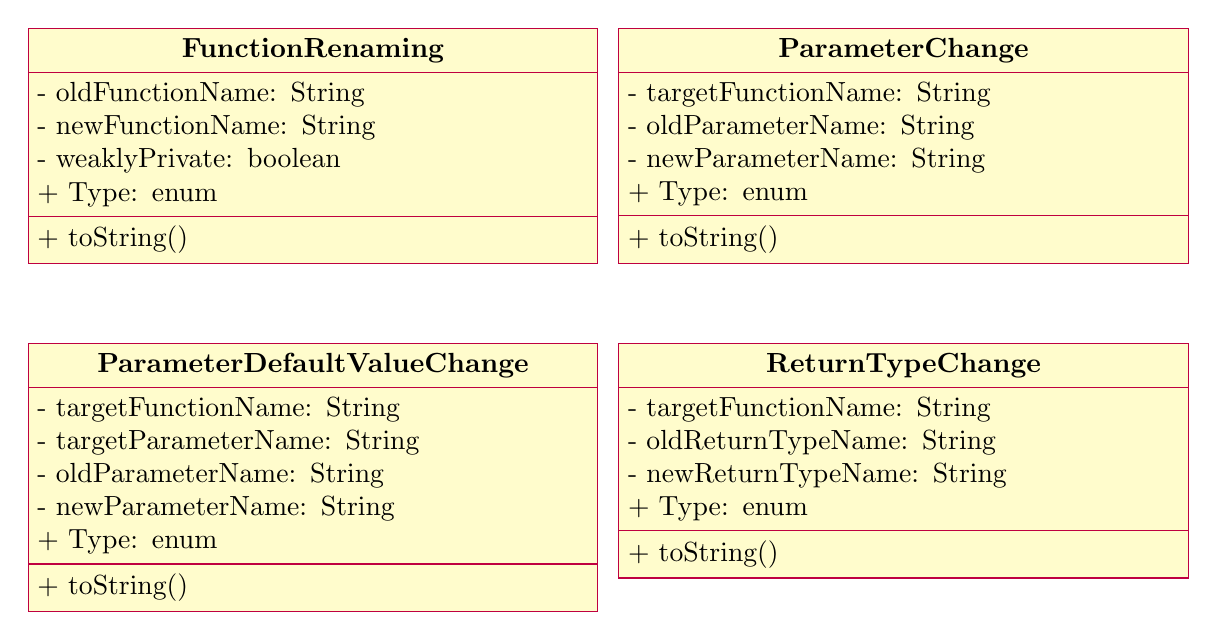
\begin{tikzpicture}
		\begin{class}[text width=7cm]{FunctionRenaming}{0,0}
			\attribute{- oldFunctionName: String}
			\attribute{- newFunctionName: String}
			\attribute{- weaklyPrivate: boolean}
			\attribute{+ Type: enum}
			\operation{+ toString()}
		\end{class}

		\begin{class}[text width=7cm]{ParameterChange}{7.5,0}
			\attribute{- targetFunctionName: String}
			\attribute{- oldParameterName: String}
			\attribute{- newParameterName: String}
			\attribute{+ Type: enum}
			\operation{+ toString()}
		\end{class}

		\begin{class}[text width=7cm]{ParameterDefaultValueChange}{0,-4}
			\attribute{- targetFunctionName: String}
			\attribute{- targetParameterName: String}
			\attribute{- oldParameterName: String}
			\attribute{- newParameterName: String}
			\attribute{+ Type: enum}
			\operation{+ toString()}
		\end{class}

		\begin{class}[text width=7cm]{ReturnTypeChange}{7.5,-4}
			\attribute{- targetFunctionName: String}
			\attribute{- oldReturnTypeName: String}
			\attribute{- newReturnTypeName: String}
			\attribute{+ Type: enum}
			\operation{+ toString()}
		\end{class}
	\end{tikzpicture}
\end{figure*}

\section{Edit Script Generation}

The edit scripts of input Python source files are generated by directly calling GumTree APIs.

\section{Change Detections}

As explained in \hyperref[chap:background]{Background}, edit actions are operations that modify the nodes or subtrees of the AST of the older file. Each edit action object in GumTree API bonds with an AST node (subtree roots for operations on subtrees). The basic idea is to traverse through the edit script produced by GumTree and inspect each edit action along with its corresponding AST node within that edit script and find the ones that match the characteristics of our identifiable changes.

A major concern is the sequential order in which we detect the four general categories of changes. As demonstrated in the skeleton algorithm, I start from changes of a larger scale gradually to smaller scales (\hyperref[fig:change-detect-routine]{Figure 4.2}). Due to the fact that it requires method information to describe a parameter or return type change, and method and parameter information to describe a parameter default value change, Collecting method and parameter change records in advance makes it possible to check if the method or parameter whose default value changed has been renamed.

\tikzstyle{block} = [rectangle, draw, text width=20em, text centered, rounded corners, minimum height=4em]
\tikzstyle{line} = [draw, very thick, -latex']
\tikzstyle{cloud} = [ellipse, draw, text width=6em, node distance=2.5cm, minimum height=2em]

% TODO: Change this figure to ppt version
\begin{figure}
	\caption{Change detection routine}
	\label{fig:change-detect-routine}
	\begin{center}
		\begin{tikzpicture}[scale=2, node distance = 2cm, auto]
			% Place nodes
			\node[block](compute){Compute edit script};
			\node[block, below of=compute](check-func-rename){Check function renaming};
			\node[block, below of=check-func-rename](check-func-relocate){Check function relocation};
			\node[block, below of=check-func-relocate](check-param){Check parameter changes};
			\node[block, below of=check-param](check-param-default-val){Check parameter default value changes};
			\node[block, below of=check-param-default-val](check-return){Check return type changes};
			% Draw edges
			\path[line](compute) -- (check-func-rename);
			\path[line](check-func-rename) -- (check-func-relocate);
			\path[line](check-func-relocate) -- (check-param);
			\path[line](check-param) -- (check-param-default-val);
			\path[line](check-param-default-val) -- (check-return);
		\end{tikzpicture}
	\end{center}
\end{figure}

\begin{figure}
	\caption{Typical AST structure of a function signature}
	\includegraphics[width=\textwidth]{ast.png}
\end{figure}

\subsection{Function Renaming Detection}
\label{subsec:func-rename-detect}

Function renaming changes are recorded in an \textit{Update} action that changes the label of the first child \textit{name} node of \textit{funcdef} node, this is to be distinguished from return annotation updates which affects the fourth child \textit{name} node of \textit{funcdef}. After locating a function renaming operation, inspecting leading underscores in the old function name as well as the new one determines the accessibility modification status.

\begin{algorithm}
	\label{algo:function-renaming-detection}
	\caption{Function renaming detection algorithm}
	\SetAlgoLined
	\begin{algorithmic}[1]
		\REQUIRE Edit script $S$ and collection of function renaming changes $R$
		\FORALL{$A \in S$}
			\STATE $node \gets$ getNode($A$);
			\IF{$A \in$ Update \\
			\AND $node \in$ name \\
			\AND getParent($node$) $\in$ funcdef \\
			\AND posInParent($node$) $= 0$}
				\STATE $old \gets$ getLabel($node$);
				\STATE $new \gets$ getValue($A$);
				\IF{$old$.startsWith("$\_$") \AND $!new$.startsWith("$\_$")}
					\STATE $record \gets$ renaming (private to public);
				\ELSIF{$new$.startsWith("$\_$") \AND $!old$.startsWith("$\_$")}
					\STATE $record \gets$ renaming (public to private);
				\ELSE
					\STATE $record \gets$ renaming (no accessibility switch);
				\ENDIF
				\STATE Append $record$ to $R$;
			\ENDIF
		\ENDFOR
	\end{algorithmic}
\end{algorithm}

\subsection{Parameter Change Detection}
\label{subsec:param-change-detect}

Parameter changes include \textit{Parameter Insertion}, \textit{Parameter Removal}, \textit{Parameter Normal Update}, and \textit{cls/self Switch}. A parameter change record in ccdetector's output includes the name of the function whose parameter changed, the old and renewed parameter names, and the specific change type (\hyperref[fig:ccdetector-class-design]{Figure 4.1}).

Python supports many kinds of special parameters other than normal ones, in Python 3 it introduced the \textit{* (a bare asterisk)} operator to be placed among parameters (\hyperref[lst:asterisk-op]{Figure 4.4}), indicating that all parameters before this asterisk require positional arguments, while all parameters after it require keyword arguments.

\begin{figure}[!t]
	\lstinputlisting[
		language=diff,
		caption={Bare asterisk operator \& None default value},
		label={lst:asterisk-op}
	]{code_snippets/asterisk_operator.diff}
	\vspace{-5mm}
\end{figure}

\begin{enumerate}
	\item \textbf{Parameter Insertion/Removal} Normally, these records are stored in \textit{TreeInsert} and \textit{TreeDelete} actions that operate on a subtree rooted at a \textit{param} node. In the special scenarios of inserting or deleting an \textit{*} operator in the function signature, the edit script generated by GumTree would store an \textit{Insert}/\textit{Delete} action that deals with a single \textit{operator} node under the \textit{parameters} parent.
	\item \textbf{Parameter Update} This kind of changes are indicated by an \textit{Update} action that changes the label of the child \textit{name} node under \textit{param} parent. Further investigations of whether the two involved names are cls and self will decide that this update is a normal one or a cls/self switch.
\end{enumerate}

ccdetector automatically checks if the target function of a parameter change operation has been renamed in the findings of \hyperref[subsec:func-rename-detect]{Function Renaming Detection}, and record the current name of the target function.

\begin{algorithm}
	\label{algo:parameter-change-detection}
	\caption{Parameter change detection algorithm}
	\begin{algorithmic}[1]
		\REQUIRE Edit script $S$ and collection of parameter changes $R$
		\FORALL{$A \in S$}
			\STATE $node \gets$ getNode($A$);
			\IF{$A \in$ TreeInsert
			\AND $node \in$ param}
				\STATE $record \gets$ parameter insertion;
			\ELSIF{$A \in$ TreeDelete
			\AND $node \in$ param}
				\STATE $record \gets$ parameter removal;
			\ELSIF{$A \in$ Insert
			\AND getParent($node$) $\in$ parameters \\
			\AND $node \in$ operator
			\AND getLabel($node$) $= *$}
				\STATE $record \gets$ parameter insertion;
			\ELSIF{$A \in$ Delete
			\AND getParent($node$) $\in$ parameters \\
			\AND $node \in$ operator
			\AND getLabel($node$) $= *$}
				\STATE $record \gets$ parameter removal;
			\ELSIF{$A \in$ Update}
				\STATE $old \gets$ getLabel($node$);
				\STATE $new \gets$ getValue($A$);
			\IF{$old =$ cls \AND $new =$ self \OR \\
				$old =$ self \AND $new =$ cls}
					\STATE $record \gets$ cls/self switch;
				\ELSE
					\STATE $record \gets$ normal update;
				\ENDIF
			\ENDIF
			\STATE Append $record$ to $R$;
		\ENDFOR
	\end{algorithmic}
\end{algorithm}

\subsection{Parameter Default Value Change Detection}

Parameter default value changes include \textit{Parameter Default Value Addition}, \textit{Parameter Default Value Removal}, and \textit{Parameter Default Value Update}. The data types of the default values are generally divided into three categories:

\begin{itemize}
	\item \textbf{Primitive types} Strings and numeric data types are stored in single AST nodes, relating to Insert, Delete, and Update edit actions.
	\item \textbf{\textit{Lists}, \textit{Dictionaries}, and container types} These values are represented as subtrees rooted at an \textit{atom} node. Addition, removal, and even update operations on these values usually involve tree edit actions TreeInsert and TreeDelete.
	\item \textbf{\textit{None}} The \textit{None} default value is worth additional attention as there are no AST nodes defined for it by GumTree's parser. Modifications related to it are still traceable though, as Update actions operate on existing AST nodes, and the addition and removal of default value nodes always occur alongside the same operation of the delimiter (an \textit{operator} node whose label is a comma symbol) before them. So adding or removing a comma operator under a param parent would be regarded as adding or removing a \textit{None} default value, and adding or removing a comma operator following a value node would be regarded as adding or removing a normal default value.
\end{itemize}

A parameter default value change record's attributes contain the names of the function and parameter locating the spot of the changed default value, the previous and current value stored in strings, as well as the specific subdivided change category (\hyperref[fig:ccdetector-class-design]{Figure 4.1}).

\begin{enumerate}
	\item \textbf{Parameter Default Value Addition/Removal} These changes are usually stored in a \textit{Insert}/\textit{Delete} action that adds or removes a single child node of \textit{param} nodes, but there are some special cases to be considered:
	\begin{enumerate}
		\item \textbf{Affilated with parameter insertion/removal} Default values might come and go with their parameters as collateral effects in parameter insertions/removals. Essentially, we could review the parameter insertion/removal records obtained in \hyperref[subsec:param-change-detect]{Parameter Change Detection}, and check if the inserted/removed subtree rooted at a \textit{param} node contains default values.
		\item \textbf{The \textit{None} value}
	\end{enumerate}
	\item \textbf{Parameter Default Value Update} Unlike separating normal parameter updates from cls/self switches, updating a parameter default value with a new value of the same or different data type will not change the subdivided category of the operation. Though they do require different detection techniques.
	\begin{enumerate}
		\item \textbf{Same data type} This will be stored in an \textit{Update} edit action that alters the label of a default value node.
		\item \textbf{Different data type} This will be recorded as two separated edit actions, one removing the obsolete default value node from the AST and one adding the node of the new default value at the same spot. This change cannot be detected in one move because it is impossible to tell a default value addition/removal operation from one of these by inspecting only one action. The only distinguishing factor is that the two actions in this change operate under the same \textit{param} parent node. In the edit script generated by GumTree, \textit{Insert} actions are listed before \textit{Delete} actions. So we collect all the added nodes in Insert actions in a list, and seek for matches when processing the sequence of Delete actions in the edit script (\hyperref[algo:check-param-update-remove]{Algorithm 4.4}). On finding a matched pair of nodes of Insert and Delete actions, add a default value update to the records, otherwise, we have found a default value removal. After exhausting actions in the edit script, the remaining added nodes in the list are of default value addition.
	\end{enumerate}
\end{enumerate}

\begin{algorithm}
	\caption{Parameter default value change detection algorithm}
	\begin{algorithmic}[1]
		\REQUIRE Edit script $S$, collection of parameter insertions $I$, collection of parameter deletions $D$, collection of added nodes $A$, collection of removed nodes $M$, and collection of parameter default value changes $R$
		\FORALL{$pi \in I$ $pd \in D$}
			\STATE $node \gets$ getNode($pi$);
			\IF{getChildrenSize($node$) > 2}
				\STATE Add a parameter default value addition record to $R$;
			\ENDIF
			\STATE $node \gets$ getNode($pd$);
			\IF{getChildrenSize($node$) > 2}
				\STATE Add a parameter default value addition record to $R$;
			\ENDIF
		\ENDFOR
		\STATE $addedNodes \gets$ []
		\STATE $removedNodes \gets$ []
		\FORALL{$A \in G$}
			\STATE $node \gets$ getNode($A$);
			\IF{$A \in$ TreeInsert
			\AND getParent($node$) $\in$ param \\
			\AND $node \in$ atom}
				\STATE Add $node$ to $addedNodes$;
			\ELSIF{$A \in$ TreeDelete
			\AND getParent($node$) $\in$ param \\
			\AND $node \in$ atom}
				\STATE checkParameterDefaultValueRemovalUpdate($node$);
			\ELSIF{$A \in$ Insert
			\AND getParent($node$) $\in$ param \\
			\AND $node \in$ (string | number)}
				\STATE Add $node$ to $addedNodes$;
			\ELSIF{$A \in$ Delete
			\AND getParent($node$) $\in$ param \\
			\AND $node \in$ (string | number)}
				\STATE checkParameterDefaultValueRemovalUpdate($node$);
			\ELSIF{$A \in$ Update
			\AND getParent($node$) $\in$ param \\
			\AND getName($node$) = "name"}
				\STATE Add a parameter default value update record to $R$;
			\ENDIF
		\ENDFOR
		\FORALL{$a \in A$}
			\STATE Add a parameter default value addition record to $R$;
		\ENDFOR
		\FORALL{$m \in M$}
			\STATE Add a parameter default value removal record to $R$;
		\ENDFOR
	\end{algorithmic}
\end{algorithm}

\begin{algorithm}
	\caption{Check for parameter default value update/removal}
	\label{algo:check-param-update-remove}
	\begin{algorithmic}[1]
		\REQUIRE Action node $n$, collection of added nodes $A$, collection of removed nodes \\
		$M$, and collection of parameter default value changes $R$
		\STATE $b \gets False$;
		\FORALL{$a \in A$}
			\IF{(getParamName($n$) = getParamName($a$) \\
			\AND getFuncName($n$) = getFuncName($a$)) \\
			\OR getPos($n$) = getPos($a$)}
				\STATE Add a parameter default value update record to $R$;
				\STATE Remove $a$ from $A$;
				\STATE $b$ = $True$;
			\ENDIF
		\ENDFOR
		\IF{$b$ = $False$}
			\STATE Add $n$ to $M$;
		\ENDIF
	\end{algorithmic}
\end{algorithm}

\subsection{Return Type Change Detection}

Return annotations are type hints in the function signature indicating the type of the value returned by the function. Checking for return annotation changes is akin to a simplified process of checking parameter default value changes. The AST node of return annotation is a \textit{name} node under \textit{funcdef} parent, at the same level as \textit{parameters} which is the parent of all parameter (\textit{param}) nodes (\hyperref[algo:return-change-detect]{Algorithm 4.5}). There are generally three types: \textit{Return Type Addition}, \textit{Return Type Removal}, and \textit{Return Type Update}.

\begin{algorithm}
	\caption{Return type change detection algorithm}
	\label{algo:return-change-detect}
	\begin{algorithmic}[1]
		\REQUIRE Edit script $S$, collection of added nodes $A$, collection of removed nodes \\
		$M$, and collection of return type changes $R$
		\FORALL{$A \in S$}
			\STATE $node \gets$ getNode($A$);
			\IF{$node \in$ name
			\AND getParent($node$) $\in$ funcdef \\
			\AND getPosInParent($node$) = 3}
				\IF{$A \in$ Insert}
					\STATE Add a return type addition record to $R$;
				\ELSIF{$A \in$ Delete}
					\STATE Add a return type removal record to $R$;
				\ELSIF{$A \in$ Update}
					\STATE Add a return type update record to $R$;
				\ENDIF
			\ENDIF
		\ENDFOR
	\end{algorithmic}
\end{algorithm}

\chapter{Tool Evaluation}
\label{chap:tool-evaluation}

This is tool evaluation.

% \chapter{Discussions}
\label{chap:discussions}

\section{The \textit{*args} and \textit{**kwargs} Parameters}

Besides \textit{* (bare asterisk)}, other special parameters in Python functions include \textit{*args} and \textit{**kwargs}, both enabling programmers to pass a variable number of arguments to a function, whose content cannot be retrieved by merely looking at the function signature. The former allows passing a list of parameters, possibly of different types, into the function. The latter contains a dictionary of parameters.

Modifications related to the two variable-quantity-parameter symbols are extra tricky to deal with, as the contents of those two parameters would only be unmasked by comprehending the actual implementation in the function body. If the framework API developer decided to insert or remove variables inside \textit{*args} or \textit{**kwargs}, or change the type of internal variables, we could only know until they take effects.  As previously explained, the analysis in this project is completely based on the edit scripts generated by GumTree. And currently, the inspection stays at the function signature level, not digging into detailed implementation. In addition, type analysis is also tremendously helpful but difficult and yet to be carried out. Based on the above reasons, ccdetector leaves the analysis of \textit{*args} and \textit{**kwargs} to future endeavors.

\section{\textit{Boolean} Values}

As one of Python's built-in types, booleans are subtypes of integers. The obstacle of analyzing it lies in that its node is found missing at the location of a boolean value in the AST produced by GumTree's parser. Due to this unexpected behavior, \textit{ccdetector} is currently not able to detection boolean-value-related modifications.

\section{Cross-file Function Relocation}

Due to the limitation that the evolution of only one Python source file is analyzed at a time, function relocations from the original file to others are not detected.

\chapter{Conclusion}
\label{chap:conclusion}

In this thesis, we conducted an empirical study of commit histories of real-world Python frameworks to understand the high-level compound changes in Python framework API evolution. We collected 535 commits that represented typical compound change patterns in three popular Python libraries. Based on our empirical findings, we designed and implemented a tool that can automatically detect compatibility issues in client programs caused by compound breaking changes in dependent Python frameworks. \textit{And will evaluate it on real-world projects to measure its capability.}


\backmatter

\bibliographystyle{sustcbib}%{GBT7714-2005NLang-UTF8}
\bibliography{bib/tex}
\nocite{*} % for every item
\begin{thanks}

This is ackowledgement.

\vskip 18pt

\begin{flushright}

Junda Ai

March, 2021

\end{flushright}

\end{thanks}


\end{document}
